\documentclass[english,,man]{apa6}
\usepackage{lmodern}
\usepackage{amssymb,amsmath}
\usepackage{ifxetex,ifluatex}
\usepackage{fixltx2e} % provides \textsubscript
\ifnum 0\ifxetex 1\fi\ifluatex 1\fi=0 % if pdftex
  \usepackage[T1]{fontenc}
  \usepackage[utf8]{inputenc}
\else % if luatex or xelatex
  \ifxetex
    \usepackage{mathspec}
  \else
    \usepackage{fontspec}
  \fi
  \defaultfontfeatures{Ligatures=TeX,Scale=MatchLowercase}
\fi
% use upquote if available, for straight quotes in verbatim environments
\IfFileExists{upquote.sty}{\usepackage{upquote}}{}
% use microtype if available
\IfFileExists{microtype.sty}{%
\usepackage{microtype}
\UseMicrotypeSet[protrusion]{basicmath} % disable protrusion for tt fonts
}{}
\usepackage{hyperref}
\hypersetup{unicode=true,
            pdftitle={Visualising two approaches to explore reliability-power relationships},
            pdfauthor={Sam Parsons},
            pdfkeywords={reliability, statistical power},
            pdfborder={0 0 0},
            breaklinks=true}
\urlstyle{same}  % don't use monospace font for urls
\ifnum 0\ifxetex 1\fi\ifluatex 1\fi=0 % if pdftex
  \usepackage[shorthands=off,main=english]{babel}
\else
  \usepackage{polyglossia}
  \setmainlanguage[]{english}
\fi
\usepackage{graphicx,grffile}
\makeatletter
\def\maxwidth{\ifdim\Gin@nat@width>\linewidth\linewidth\else\Gin@nat@width\fi}
\def\maxheight{\ifdim\Gin@nat@height>\textheight\textheight\else\Gin@nat@height\fi}
\makeatother
% Scale images if necessary, so that they will not overflow the page
% margins by default, and it is still possible to overwrite the defaults
% using explicit options in \includegraphics[width, height, ...]{}
\setkeys{Gin}{width=\maxwidth,height=\maxheight,keepaspectratio}
\IfFileExists{parskip.sty}{%
\usepackage{parskip}
}{% else
\setlength{\parindent}{0pt}
\setlength{\parskip}{6pt plus 2pt minus 1pt}
}
\setlength{\emergencystretch}{3em}  % prevent overfull lines
\providecommand{\tightlist}{%
  \setlength{\itemsep}{0pt}\setlength{\parskip}{0pt}}
\setcounter{secnumdepth}{0}
% Redefines (sub)paragraphs to behave more like sections
\ifx\paragraph\undefined\else
\let\oldparagraph\paragraph
\renewcommand{\paragraph}[1]{\oldparagraph{#1}\mbox{}}
\fi
\ifx\subparagraph\undefined\else
\let\oldsubparagraph\subparagraph
\renewcommand{\subparagraph}[1]{\oldsubparagraph{#1}\mbox{}}
\fi

%%% Use protect on footnotes to avoid problems with footnotes in titles
\let\rmarkdownfootnote\footnote%
\def\footnote{\protect\rmarkdownfootnote}


  \title{Visualising two approaches to explore reliability-power relationships}
    \author{Sam Parsons\textsuperscript{1}}
    \date{}
  
\shorttitle{Visualising reliability-power relationships}
\affiliation{
\vspace{0.5cm}
\textsuperscript{1} University of Oxford}
\keywords{reliability, statistical power\newline\indent Word count: 2979}
\usepackage{csquotes}
\usepackage{upgreek}
\captionsetup{font=singlespacing,justification=justified}

\usepackage{longtable}
\usepackage{lscape}
\usepackage{multirow}
\usepackage{tabularx}
\usepackage[flushleft]{threeparttable}
\usepackage{threeparttablex}

\newenvironment{lltable}{\begin{landscape}\begin{center}\begin{ThreePartTable}}{\end{ThreePartTable}\end{center}\end{landscape}}

\makeatletter
\newcommand\LastLTentrywidth{1em}
\newlength\longtablewidth
\setlength{\longtablewidth}{1in}
\newcommand{\getlongtablewidth}{\begingroup \ifcsname LT@\roman{LT@tables}\endcsname \global\longtablewidth=0pt \renewcommand{\LT@entry}[2]{\global\advance\longtablewidth by ##2\relax\gdef\LastLTentrywidth{##2}}\@nameuse{LT@\roman{LT@tables}} \fi \endgroup}


\DeclareDelayedFloatFlavor{ThreePartTable}{table}
\DeclareDelayedFloatFlavor{lltable}{table}
\DeclareDelayedFloatFlavor*{longtable}{table}
\makeatletter
\renewcommand{\efloat@iwrite}[1]{\immediate\expandafter\protected@write\csname efloat@post#1\endcsname{}}
\makeatother
\usepackage{float}
\usepackage{caption}
\floatplacement{figure}{H}
\raggedbottom

\authornote{I would like to thank Anne-Wil Kruijt for her input on the original code used to generate Figure 1 in an earlier version of this paper.
The code used to run the simulations and generate this paper can be found in the OSF repository for this paper \url{https://osf.io/msk2w/}
The author is currently supported by a grant from the Economic and Social Research Council {[}grant ref: ES/R004285/1{]}

Correspondence concerning this article should be addressed to Sam Parsons, Department of Experimental Psychology, University of Oxford, New Radcliffe House, Radcliffe Observatory Quarter, Oxford, OX2 6AE. E-mail: \href{mailto:sam.parsons@psy.ox.ac.uk}{\nolinkurl{sam.parsons@psy.ox.ac.uk}}}

\abstract{
The relationship between measurement reliability and statistical power is a complex one. Where reliability is defined by classical test theory as the proportion of `true' variance to total variance (the sum of true score and error variance), power is only functionally related to total variance. Therefore, to explore direct relationships between reliability and power, one must fix either true-score variance or error variance while varying the other. Here, visualisations are used to illustrate the reliability-power relationship under conditions of fixed true-score variance and fixed error variance. From these visualisations, conceptual distinctions between fixing true-score or error variance can be raised. Namely, that when true-score variance is fixed, low reliability (and low power) represents error hiding true effects. Whereas, when error variance is fixed, high reliability (and low power) represents a very small effect. I raise several observations I hope will be useful in considering the utility of measurement reliability and it's relationship to effect sizes and statistical power.


}

\begin{document}
\maketitle

As defined by classical test theory, observed-score variance, or \enquote{total} variance is the sum of \enquote{true-score} variance and \enquote{error} score variance (X = T + E). Measurement reliability is defined as the proportion of variance attributed to true-score relative to total variance (R = T / T+E). Statistical power is the probability of detecting a specified effect size, or greater, at a given sample size and alpha. Statistical power is functionally related to total variance, such that increased total variance results in a reduction in power. Thus, power is related to total variance, regardless of how it is split into true-score and error variance. It follows that reliability does not therefore have a direct functional relationship with power. That is, unless either true-score variance or error variance is held constant while the other is left to vary; as Zimmerman and Zumbo (2015) have demonstrated clearly. By varying only true-score or only error variance; total variance varies in proportion and we can examine the ensuing relationship between reliability and power. Briefly, when true variance is fixed, increases in error variance result in decreases in reliability and decreases in statistical power. In contrast, fixing error variance and increasing true variance results in increases in reliability, yet, this is accompanied by a decrease in power. Zimmerman and Zumbo (2015) provide an excellent coverage of the mathematical definitions underlying these relationships; and I do not aim to simply repeat them in this paper. Instead, I present these relationships visually comparing a hypothetical measure with zero, the research question being, simply, does the group differ significantly from zero? First, total variance is fixed while true-score and error variance alternate. Second, true-score variance is fixed, while error variance is increased. Third, error variance is fixed, while true-score variance is increased. For each approach I describe the resulting relationship between reliability and power. I aim to highlight some of the implications that have been drawn from either approach. Finally, I aim to highlight conceptual differences between the approaches of fixing true-score or fixing error variance. These differences may offer additional insight into interpreting results, and in particular concerning the question of whether low reliability may be a boost in experimental research.

\hypertarget{holding-total-observed-variance-constant}{%
\subsection{Holding total observed variance constant}\label{holding-total-observed-variance-constant}}

To visualise the relationships between reliability and power figure 1 presents a somewhat abnormal kind of plot. The proportion of the line in blue represents the proportion of \enquote{true-score} variance, while the proportion in red line represent the proportion of \enquote{error} variance. Total variance is therefore the total width of the line; the wider the line overall, the smaller the effect size. The reliability of the measure is presented on the y axis. For the purposed of this visualisation, we might consider lines that do not cross zero on the x axis to be significantly different from zero.

First, an illustration of no relationship between reliability and power. In the left panel of Figure 1, total variance is held constant. As the proportion of true score to error score variance reduces, the reliability of the measure also reduces. However, the effect size remains constant demonstrating that effect size is influenced by the total variance, not the proportion of that variance that is attributable to true-score and error variance.

\begin{figure}[H]
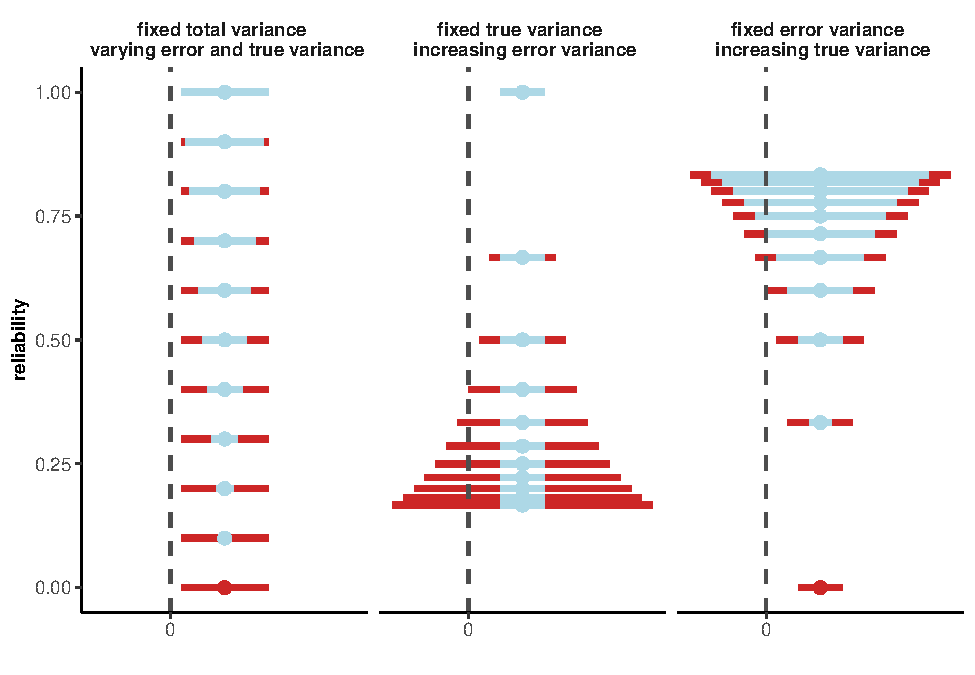
\includegraphics{visualising-reliability-and-power-relationships-v2_files/figure-latex/plotting1-1} \caption{Visualising total variance decomposition into true-score variance (blue) and error variance (red). Reliability. The reliability (true variance / total variance) is indicated on the y axis. Left panel: total variance is held constant. Middle panel: true-score variance is held constant. Right panel: error variance is held constant}\label{fig:plotting1}
\end{figure}

This is also demonstrated in Figure 2, in which power does not vary in relation to reliability. Figure 2 was generated by simulating datasets in which the error variance and true variance were alternated between 0 and 1, in .1 increments, while holding total variance constant at 1. The group mean was set to .3. Sample sizes of 20, 30, 40, 50, and 60 were generated. 20000 iterations of this 11*5 design were performed. Statistical power was then calculated as the percentage of significant results at an alpha of .05.

\begin{figure}[H]
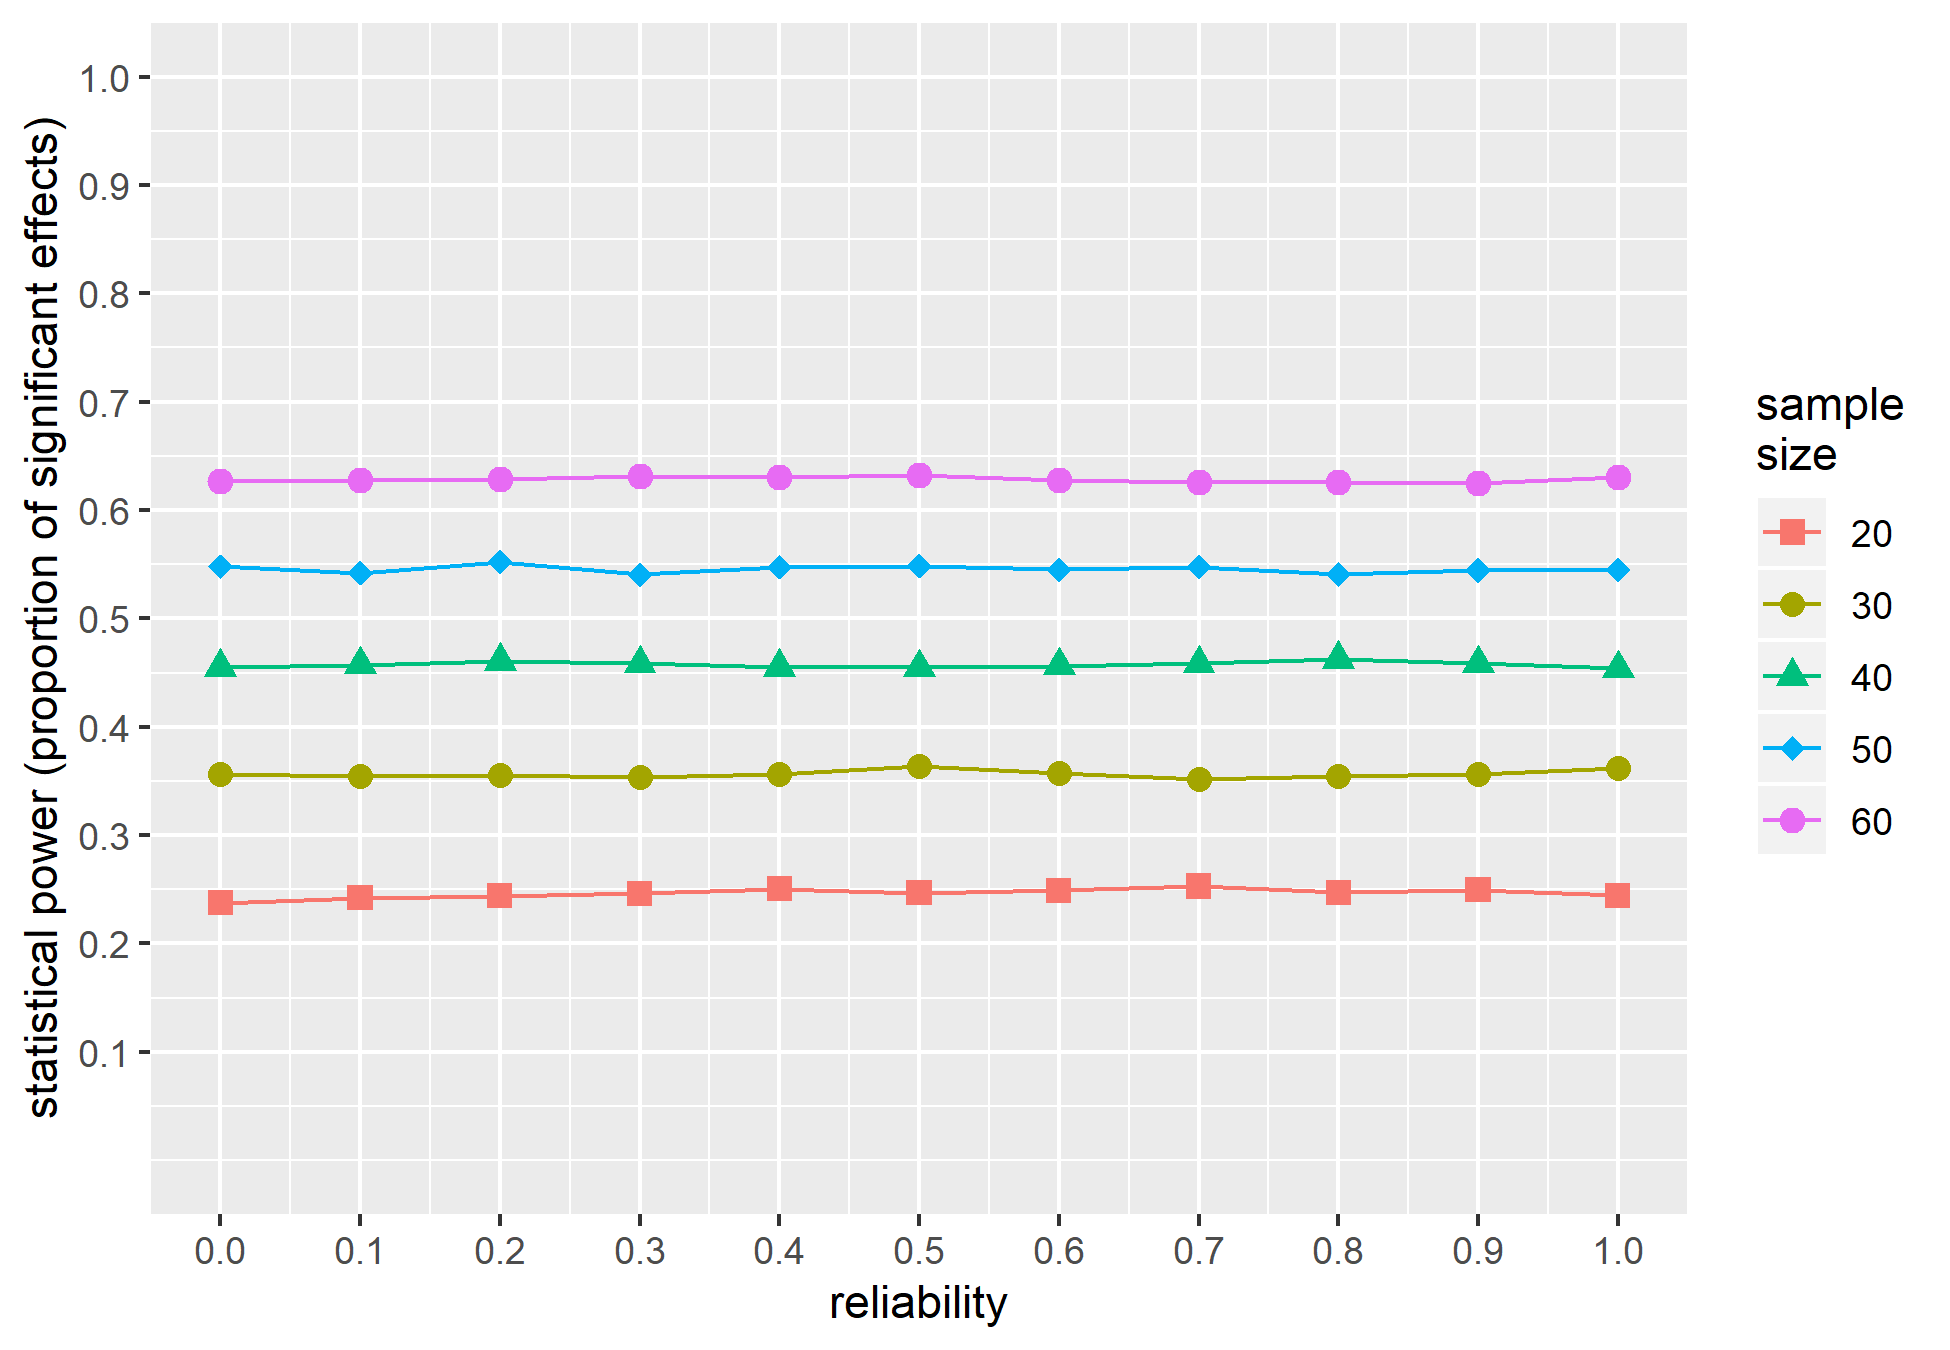
\includegraphics{visualising-reliability-and-power-relationships-v2_files/figure-latex/plotting2-1} \caption{Observed probability of finding a significant result as a function of sample size and reliability where total variance is fixed (true-score and error variance alternate)}\label{fig:plotting2}
\end{figure}

\hypertarget{increasing-error-variance}{%
\subsection{Increasing error variance}\label{increasing-error-variance}}

An often employed method to examine the relationship between reliability and power is to manipulate reliability by increasing the amount of measurement error. For instance, LeBel and Paunonen (2011) used this procedure and concluded that reductions in reliability reduce the confidence we should place in our analyses and in statistical power (and later extend this to replicability of results). Similarly, Kanyongo and colleagues (Kanyongo, Brooks, Kyei-Blankison, \& Gocmen, 2007) used a Monte Carlo simulation approach (MC2G software; \url{http://www.ohiouniversityfaculty.com/brooksg/}) to demonstrate that increasing measurement error (and therefore, reducing reliability) decreases power for specific analyses, including; paired t-tests, independent t-tests, one-way ANOVA (three groups), Wilcoxon signed-rank tests, and Mann-Whitney-Wilcoxon tests. When applied to correlational analyses, the decline in statistical power (and increase in required sample sizes to achieve 80\% power) even at \enquote{acceptable} levels of reliability is daunting (Parsons, 2018) in particular given that measurement reliability of cognitive measures often goes unreported (Gawronski, Deutsch, \& Banse, 2011; Parsons, Kruijt, \& Fox, 2019).

Figure 1 (middle panel) displays this visually by setting true variance at 1 and increasing error variance such that reliability decreases (from top to bottom) in steps of 0.1. Here, with decreases in reliability comes a decrease in the observed effect size, as the total variance increases. For the sake of interpretation, we might interpret lines that cross zero as being non-significantly different from zero. With enough added error variance, even real effects will be hidden.

To illustrate the relationship between reliability and power under the assumption of fixed true-score variance, simulated data were generated following Lebel and Paunonen's (2011) approach. True variance was set at 1, and error variance increased such that reliability decreased from 1 to .1 in steps of .1. The group average was set to .3. Sample sizes of 20, 30, 40, 50, and 60 per group were created. 20000 iterations of this 10*5 design were performed. Statistical power was calculated as the percentage of significant results at an alpha of .05. Figure 3 presents this visually. Note that this plot closely matches the one created by Lebel and Paunonen (2011, p.~576).

\begin{figure}[H]
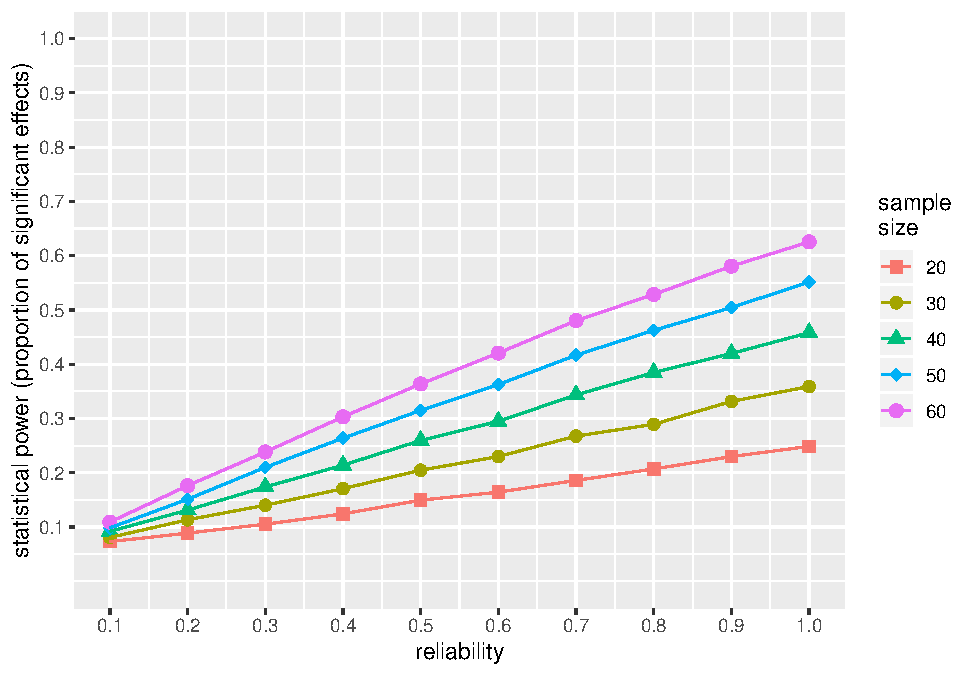
\includegraphics{visualising-reliability-and-power-relationships-v2_files/figure-latex/plotting3-1} \caption{Observed probability of finding a significant result as a function of sample size and reliability where truescore is fixed and error variance is increased}\label{fig:plotting3}
\end{figure}

\hypertarget{increasing-true-score-variance}{%
\subsection{Increasing true-score variance}\label{increasing-true-score-variance}}

The alternative approach to examine the relationship between reliability and power is to fix error variance and vary true variance (De Schryver, Hughes, Rosseel, \& De Houwer, 2016; Zimmerman \& Zumbo, 2015). In this case the reverse pattern to fixing true-score variance is observed; power decreases with increased reliability when error variance is held constant. Figure 1 (right panel) displays this visually by setting error variance at 1 and increasing true-score variance such that reliability increases (from top to bottom) in steps of 0.1. Here, with increased true-score variance comes increases in reliability co-occurring with decreases in the observed effect size. Thus, the more reliable measure here also coincides with the lowest power.

As with the previous approach, data were simulated to illustrate the relationship between reliability and power, assuming that error variance is fixed. In this case, error variance was set to 1 and true variance was increased such that reliability varied from 0 to .9 in steps of .1. The mean group score was set to .3. Sample sizes of 20, 30, 40, 50, and 60 were created. 20000 iterations of this 10*5 design were performed. Statistical power was calculated as the percentage of significant results at an alpha of .05. Figure 4 presents this visually. Note that this plot closely matches the one created by De Schryver et al.~(2016, p.~4). Here, we observe that power and reliability have an inverse relationship.

\begin{figure}[H]
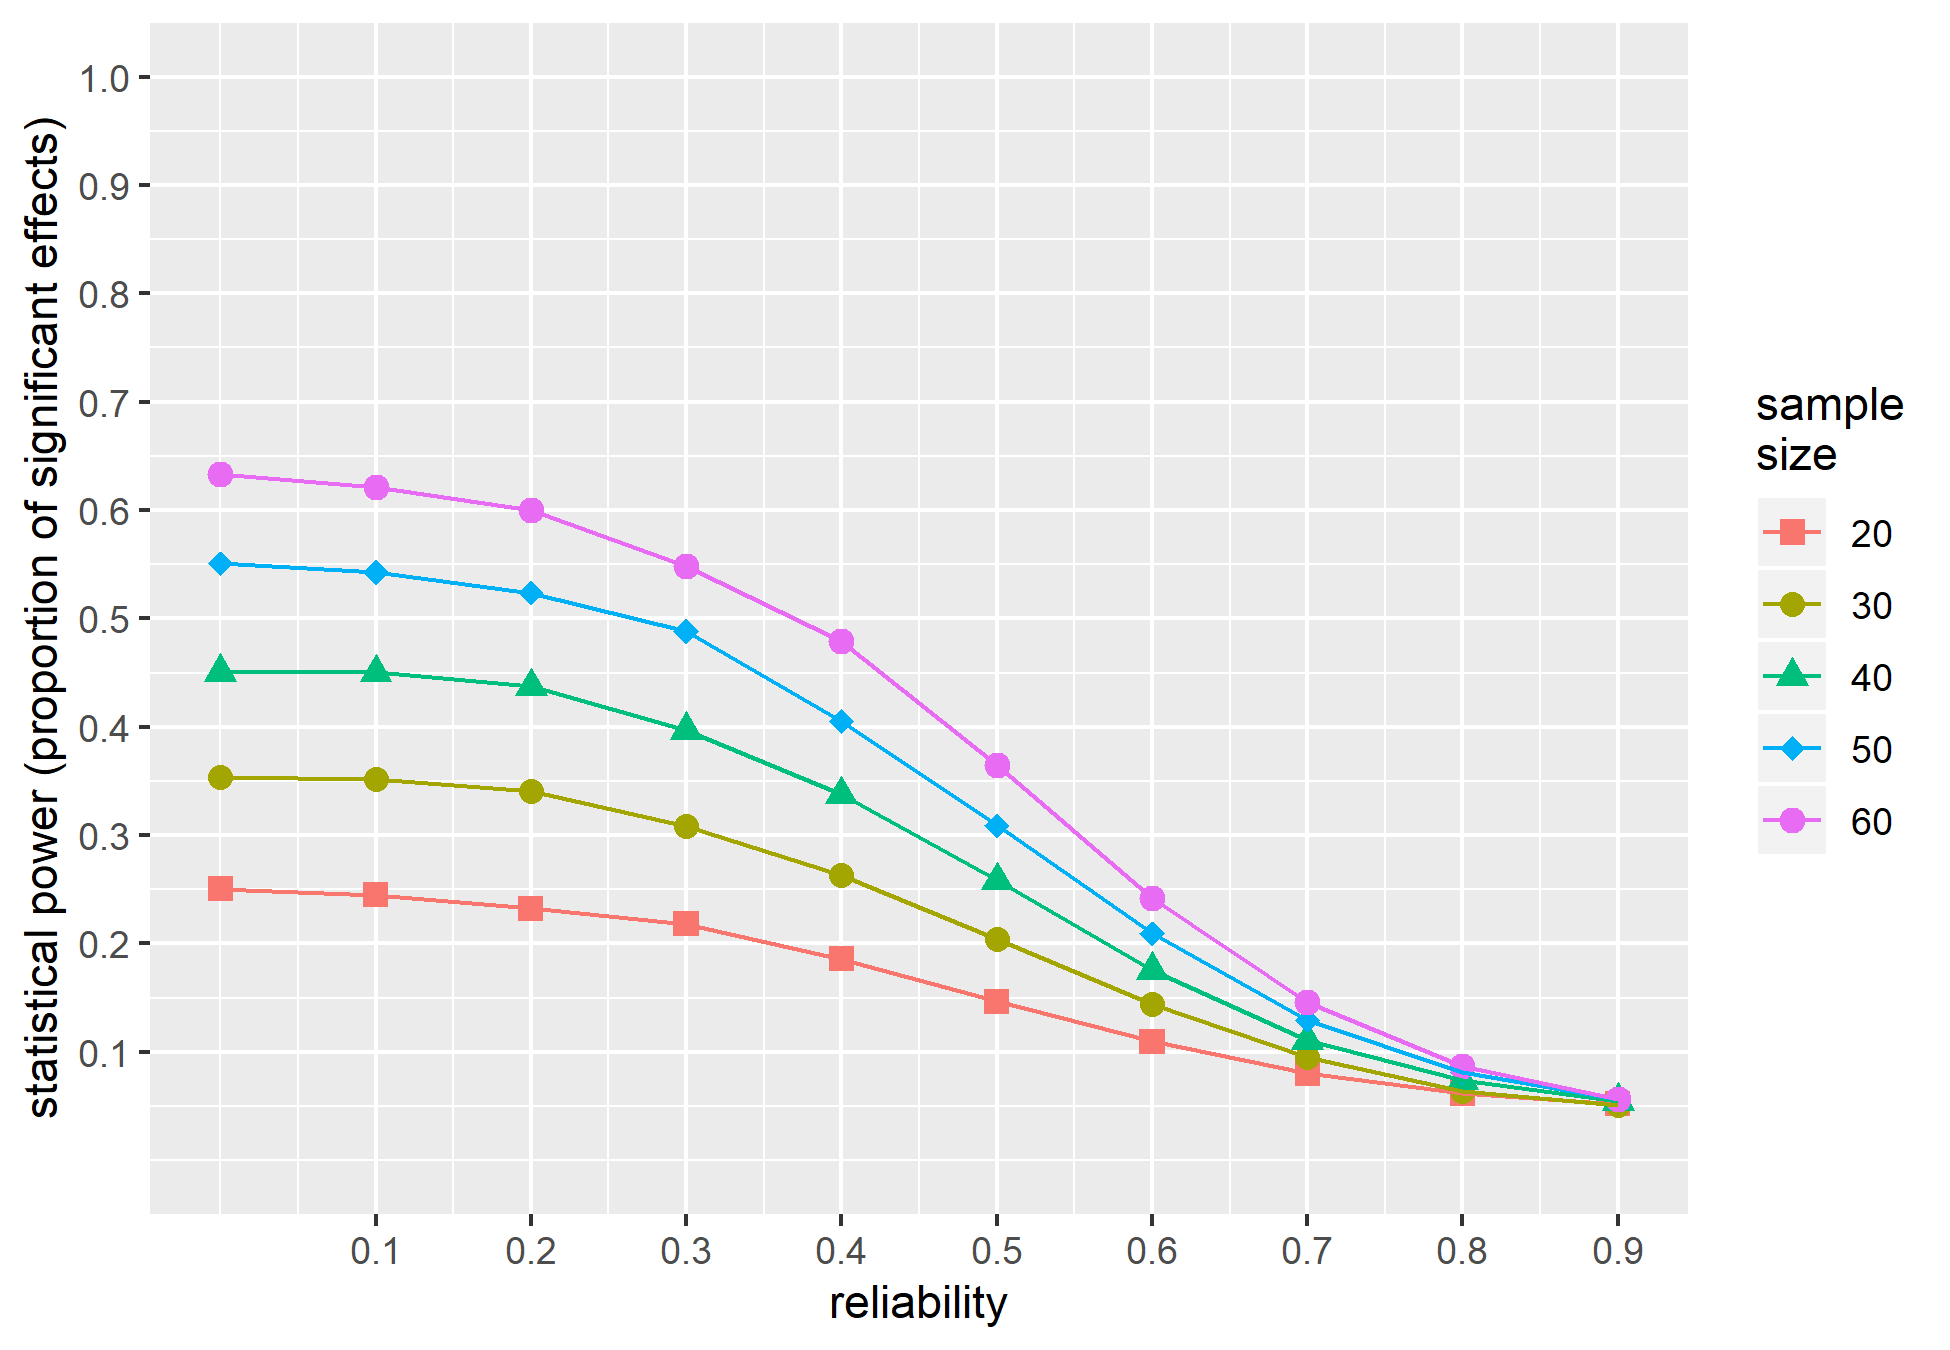
\includegraphics{visualising-reliability-and-power-relationships-v2_files/figure-latex/plotting4-1} \caption{Observed probability of finding a significant result as a function of sample size and reliability where error is fixed and truescore variance is varied.}\label{fig:plotting4}
\end{figure}

\hypertarget{interpreting-different-reliability-power-relationships}{%
\subsection{Interpreting different reliability-power relationships}\label{interpreting-different-reliability-power-relationships}}

The relationship between measurement reliability and statistical power is complex, in so far as it is not a direct relationship. To examine a direct, functional, relationship between reliability and power, either true-score variance or error variance must be fixed, while the other is held constant. Following mathematical definitions is useful in examining the reliability-power relationship (Zimmerman \& Zumbo, 2015). Here, I aimed to supplement previous articles with visualisations of the reliability-power relationship with the aim of elucidating the implications of either assummption. Under either assumption, increases in either true-score variance or error variance lead to an increase in total variance and a direct reduction in statistical power. As demonstrated above, adopting the approach of fixing true-score variance (LeBel \& Paunonen, 2011) leads to a positive relationship between reliability and power, whereas fixing measurement error (e.g.~De Schryver et al., 2016) results in an inverse relationship between measurement reliability and power.

In part, what prompted this paper were discussions about the relevance of measure reliability in different research contexts. As noted by Hedge and colleagues (2017, p.~3) \enquote{the meanings of a \enquote{reliable} task for experimental and correlational research are not only different, but can be opposite in this critical sense} due to the relative advantage or disadvantage of larger variation in the within-subject effect. Fixing true variance has led to recommendations that we must improve the psychometric properties of our measurements, so as not to render our results uninterpretable and to increase the replicability of our research (LeBel \& Paunonen, 2011; also see, Hedge, Powell, \& Sumner, 2017; Parsons, 2018; Parsons et al., 2019; Rodebaugh et al., 2016). In contrast, the approach of fixing error variance and increasing true-score variance has been related to the idea that experimentalists seek to maximise an experimental effect (and have greater statistical power) by recruiting more homogeneous samples, fitting with the aim of reducing true-score variance, which results in reductions in reliability (De Schryver et al., 2016). How can we reconcile these opposing stances on measure reliability? I suggest that part of the reconcilation comes from discussing the conceptual distinctions resulting from holding either error or true-score variance constant.

\hypertarget{conceptual-distinctions-between-approaches-to-examine-reliability-power-relationships}{%
\subsection{Conceptual distinctions between approaches to examine reliability-power relationships}\label{conceptual-distinctions-between-approaches-to-examine-reliability-power-relationships}}

The purpose of this paper is to highlight conceptually distinct rationales for the fact that low power can result from increasing true-score variance or from error variance (while the other stays constant). Specifically, depending on the approach adopted, low power is either; a result of true effects being masked by measurement error, or a result of the effect itself being very small. Of course, I do not aim to argue against these functional relationships between reliability and power. Both rest on mathematical definitions, after all. I do, however, believe that there are conceptual considerations that must be made when interpreting the relationship between reliability and power under either assumption. These conceptualisations have implications for some claims that have been made about the importance of reliability in experimental research. (De Schryver, 2018) provides an illustrating example. Consider two measures, A and B, with error variance of .20. Score A contains true-score variance of .80 (therefore, a reliability of .80), while score B contains true-score variance of .60 (therefore, a reliability of .75). Score A is therefore preferable based on solely on reliability. Yet, calculating Cohen's d - assuming a mean difference of .50 - reveals that the effect size for A is .50 and for B is .56 due to the greater total variance in score A. Therefore, to maximise the effect size observed, a researcher might seek to use measure B. This example again highlights the fact that reliability does not have a 1:1 relationship with statistical power. Selecting a measure based on the size of the effect it produces with the aim of increasing power may be a valid approach. However, my concern is that this approach might be interpreted as an indication that low reliability is either; not a problem, or may be beneficial under certain conditions. This simplistic conclusion misses the fact that it is total variance that is functionally related to power and not reliability per se. I also worry that demonstrations of this negative relationship has led some to conclude that low reliability is therefore \enquote{acceptable} for experimental designs, and by implication that we should not be concerned about the reliability of our measures. This concern was part of what prompted creating the visualisations in this paper.

To conclude, I leave the reader with two observations based on the visualisations above that I have not yet seen articulated in discussions surrounding the relationship between reliability and power. I hope that these observations are useful in considering the utility of measurement reliability in experimental research.

First, as highlighted in figure 1; for any specified level of total variance, reliability can take any value. In this case, regardless of reliability; power remains constant despite reductions in the \enquote{meaning} of the scores on an individual differences level. While this reduction in reliability does not influence the power of the between group difference, it does influence correlational analyses with this measure as individuals become harder to rank order. Likewise, it would be difficult to demonstrate that an individual's score has changed or to investigate questions of individual differences. Further, it has been recently argued that the upper bound of validity of a measure is it's reliability (Zuo, Xu, \& Milham, 2019). From this perspective, it is much more difficult to assume that one is measuring the process of interest, even with a highly powered test showing a large effect (e.g.~in Figure 1, right panel). Thus, while an effect can certainly be found, the reliability and validity of that measurement can still be suspect.

In these cases, although a highly powered systematic effect has been observed, we cannot have much confidence that this difference is in the process or construct of interest. If reliability is so low that the score is rendered near-meaningless, does it matter how much more power the test has or how much larger the effect size is? Is the measure even capturing the very thing that researchers were interested in in the first place? Highly reliable measurements have the benefit that the measure is less contaminated by error and more likely to capture the process, or construct, of interest. The only potential benefit of low reliability is of maximising effect sizes under the condition that a certain amount of measurement error is expected. However, this comes with the drawback of a less interpretable measure, and follows the assumption that if there were sufficient true-score variance for a reliable measure then there would be little-to-no actual effect to find in the first instance. In all cases, reducing measurement error is beneficial to the interpretability of scores as well as increasing power (assuming that this reduction in measurement error does not co-occur with an increase in true score variance in excess of this reduction). While experimentalists seek to maximise the effect of interest by recruiting more homogeneous groups, it does not follow that low reliability itself is beneficial, only that reducing total variance (e.g.~via reducing measurement error) will maximise the effect observed.

Finally, consider the widest lines in the middle and right panels of Figure 1. These contain the maximum total variance - and thus, the lowest power of all the tests. Each suggests an alternative interpretation for the relationship between reliability and (low) power. When error variance is increased (Figure 1, middle panel), the true effect is hidden due to measurement error. Whereas, when true variance is increased (Figure 1, right panel), the actual true effect is smaller. There is simply less of an effect to find. Therefore, we should \emph{expect} low power in this case. Although total variance is the same, the composition into true-score and error variance leads to different reasons explaining the resulting low power. We should not think of the reliability-power relationship under either approach as being a direct result of reliability.

The aim of this brief paper is to expand current examinations of the relationship between reliability and statistical power (e.g.~Zimmerman \& Zumbo, 2015). Visualising these relationships under separate assumptions of fixed true-score variance and fixed error variance suggests each method represents a conceptually distinct process. We might consider each approach separately in terms of obscuring a true effect (fixing true-score variance) or reducing the size of the effect (fixing error variance). The fact that; under the first assumption power increases with improved reliability, whereas under the second assumption the opposite is observed, is less paradoxical when considering these alternative explanations. This in itself might help to avoid potential simplifications that low reliability is acceptable under certain circumstances and promote a more in depth consideration of the influence of measurement reliability on statistical power in a given study.

\pagebreak

\hypertarget{references}{%
\subsection{References}\label{references}}

\setlength{\parindent}{-0.4in}
\setlength{\leftskip}{0.4in}
\setlength{\parskip}{8pt}

\noindent

\hypertarget{refs}{}
\leavevmode\hypertarget{ref-DeSchryver2018}{}%
De Schryver, M. (2018). \emph{A psychometric analysis of choice reaction time measures} (PhD thesis). Ghent University.

\leavevmode\hypertarget{ref-DeSchryver2016}{}%
De Schryver, M., Hughes, S., Rosseel, Y., \& De Houwer, J. (2016). Unreliable yet still replicable: A comment on lebel and paunonen (2011). \emph{Frontiers in Psychology}, \emph{6}(JAN), 1--8. doi:\href{https://doi.org/10.3389/fpsyg.2015.02039}{10.3389/fpsyg.2015.02039}

\leavevmode\hypertarget{ref-Gawronski2011}{}%
Gawronski, B., Deutsch, R., \& Banse, R. (2011). Response interference tasks as indirect measures of automatic associations. In K. Klauer, C. Stahl, \& A. Voss (Eds.), \emph{Cognitive methods in social psychology} (pp. 78--123). New York, NY: Guilford.

\leavevmode\hypertarget{ref-Hedge2017}{}%
Hedge, C., Powell, G., \& Sumner, P. (2017). The reliability paradox: Why robust cognitive tasks do not produce reliable individual differences. \emph{Behavior Research Methods}. doi:\href{https://doi.org/10.3758/s13428-017-0935-1}{10.3758/s13428-017-0935-1}

\leavevmode\hypertarget{ref-Kanyongo2007}{}%
Kanyongo, G. Y., Brooks, G. P., Kyei-Blankison, L., \& Gocmen, G. (2007). Reliability and statistical power: How measurement fallibility affects power and required sample sizes for several parametric and nonparametric statistics. \emph{Journal of Modern Applied Statistical Methods}, \emph{6}(1), 81--90. doi:\href{https://doi.org/10.22237/jmasm/1177992480}{10.22237/jmasm/1177992480}

\leavevmode\hypertarget{ref-LeBel2011}{}%
LeBel, E. P., \& Paunonen, S. V. (2011). Sexy But Often Unreliable: The Impact of Unreliability on the Replicability of Experimental Findings With Implicit Measures. \emph{Personality and Social Psychology Bulletin}, \emph{37}(4), 570--583. doi:\href{https://doi.org/10.1177/0146167211400619}{10.1177/0146167211400619}

\leavevmode\hypertarget{ref-Parsons2018}{}%
Parsons, S. (2018). Ignoring measurement reliability is a real-life horror story {[}Blog post{]}. Retrieved from \url{https://medium.com/@Sam_D_Parsons/ignoring-measurement-reliability-is-a-real-life-horror-story-b98a2517db26}

\leavevmode\hypertarget{ref-Parsons2018a}{}%
Parsons, S., Kruijt, A.-w., \& Fox, E. (2019). Psychological Science needs a standard practice of reporting the reliability of cognitive behavioural measurements, 1--25. doi:\href{https://doi.org/10.17605/OSF.IO/6KA9Z}{10.17605/OSF.IO/6KA9Z}

\leavevmode\hypertarget{ref-Rodebaugh2016}{}%
Rodebaugh, T., Scullin, R., Langer, J., Dixon, D., Huppert, J., Bernstein, A., \ldots{} Lenze, E. (2016). Unreliability as a Threat to Understanding Psychopathology: The Cautionary Tale of Attentional Bias. \emph{Journal of Abnormal Psychology}, \emph{125}(6), 840--851. doi:\href{https://doi.org/10.1037/abn0000184}{10.1037/abn0000184}

\leavevmode\hypertarget{ref-Zimmerman2015}{}%
Zimmerman, D., \& Zumbo, B. (2015). Resolving the Issue of How Reliability is Related to Statistical Power: Adhering to Mathematical Definitions. \emph{Journal of Modern Applied Statistical Methods}, \emph{14}(2), 9--26. doi:\href{https://doi.org/10.22237/jmasm/1446350640}{10.22237/jmasm/1446350640}

\leavevmode\hypertarget{ref-zuo_harnessing_2019}{}%
Zuo, X.-N., Xu, T., \& Milham, M. P. (2019). Harnessing reliability for neuroscience research. \emph{Nature Human Behaviour}. doi:\href{https://doi.org/10.1038/s41562-019-0655-x}{10.1038/s41562-019-0655-x}


\end{document}
